\documentclass[11pt,a4paper,twocolumn]{scrartcl}

% Support for UTF-8 and non-English letters require the following two
\usepackage[T1]{fontenc}
\usepackage[utf8]{inputenc}
\usepackage{algorithm2e}
\usepackage{fancyvrb}
% Font packages
\usepackage[default,defaultsans,oldstyle,proportional]{lato}
\usepackage[scaled]{beramono}
\usepackage{sfmath}
% Optimized justification via improved microtypography on character level
\usepackage{microtype}
\usepackage{ragged2e}
\usepackage[none]{hyphenat} % disable all hyphenation
\setlength{\emergencystretch}{3em} % allow extra hfill, needed if hyphenation disabled
%\overfullrule=1mm % mark overfull boxes
%\usepackage{showframe} % show edges of text areas
% Page layout
\usepackage[left=15mm,right=15mm,top=15mm,bottom=20mm,
   nohead,foot=10mm]{geometry}
% Page headers

\usepackage{scrlayer-scrpage}
\usepackage{lastpage}
% Page header
\KOMAoptions{headsepline=0pt,plainheadsepline=off}
\ihead*{}
\chead*{}
\ohead*{}
% Page footer
\KOMAoptions{footsepline=0pt,plainfootsepline=off}
\ifoot*{}
\cfoot*{Page \thepage{} of \pageref*{LastPage}}
\ofoot*{}
% Text layout
\KOMAoption{parskip}{never}
\newlength{\myparindent}
\newlength{\myparskip}
\setlength{\myparindent}{0pt}
\setlength{\myparskip}{5pt plus 1pt}
\setparsizes{\myparindent}{\myparskip}{0.1\linewidth plus 1fil}
\RedeclareSectionCommand[beforeskip=6pt,afterskip=3pt,afterindent=false]{section}
\RedeclareSectionCommand[beforeskip=6pt,afterskip=-0.5em,afterindent=false]{paragraph}
\RaggedRight
% SVN metadata
\usepackage[today,revrange,nofancy]{svninfo}
\svnInfo $Id$
% Graphics
\usepackage{graphicx}
% Colour definitions
\usepackage{xcolor}
\definecolor{secondary}{HTML}{435584}
% Floats
\usepackage{subcaption}
% Listings
\usepackage{listings}
\lstset{language=C, basicstyle=\small\ttfamily,
   aboveskip=0pt, belowskip=0pt}
\usepackage{upquote} % to use correct glyphs for single-quote in verbatim
% SI units
\usepackage{siunitx}
\sisetup{per-mode = symbol, detect-all = true}
% Hyperlinks
\usepackage[
   colorlinks=true,allcolors=secondary,breaklinks=true,
   bookmarks=true,unicode=true,bookmarksopen,bookmarksnumbered]{hyperref}
\usepackage{multicol}

% Package for pseudocode.
\usepackage{algorithm2e}
% Package for inline, verbatim text (code snippets)
\usepackage{fancyvrb}
% Math environments, including align(*)
\usepackage{amsmath}

% Document-specific settings
\renewcommand\abstractname{Executive Summary}

% define a critical section block
\SetKwBlock{CritSection}{critical section}{}

% Document details
\title{Design Brief: Group 5}
\author{
   Gabriel Apap,
   Damjan Filipovic,
   Mark Mizzi
   }
\date{\svnMaxToday, Document v.\svnInfoMaxRevision}

\hypersetup{
   colorlinks   = true
}

\begin{document}

\maketitle

\abstract{%
   This document outlines the design of a DTMF encoding system based on a microcontroller board. The system described makes use of an LCD display to show the user what keys they have pressed as well as to display any messages or errors. An LED is used as an indicator of the system's state. An on-board DAC, in conjunction with an amplifier circuit and speaker are used to generate and amplify the DTMF tones.
   }

\section{Introduction}~\label{introduction}

   Dual Tone Multi Frequency (DTMF for short) encoding is a technology used to communicate with other devices over a standard analogue telephone line \cite{sl:an218}. This is mainly used for automated switchboards for calls; however, this is also used in remote control systems, telephone banking, and other applications \cite{sl:an218}.

   The technology functions by converting each of the 16 symbols on a keypad (1-9, A-D, * and \#) into a specific tone. The tone consists of a sum of two sine waves, whose frequency is determined by pairwise combination of 4 high frequencies (representing the keypad columns) and 4 low frequencies (representing the keypad rows) \cite{sl:an218}.

   The goal of this project is to implement a DTMF encoding system based on the Embedded Artists LPC4088 microcontroller board.

   Microcontrollers are designed for use in real-time systems, and hence their software stack typically does not include an operating system. Task scheduling has to be handled explicitly by the programmer, through the use of an ad-hoc scheduler and/or interrupt handlers.

   In addition, microcontrollers are generally low-cost systems with limited hardware resources, and hence require the use of low-level programming tricks to achieve efficiency and performance despite the resource constraints.
   
   The DTMF system implemented makes use of several I/O devices, including an LCD used to convey user input or settings options to the user,
   an indicator LED which turns on when the system is booted, and a keypad input device used to navigate menus or to input DTMF symbols.

   The system also has a rich user interface which offers several options. This interface is illustrated in the control flow diagram of Figure~\ref{fig:system-interface}, and will now be described.

   On boot-up, the system prompts the user to enter one of three operational modes: manual mode, quickdial mode, and settings mode.

   In manual mode, the user can input DTMF tones on the keypad, which displays the corresponding symbol on the LCD screen, and plays the appropriate DTMF tone using the DAC and attached amplifier/speaker circuit.

   In settings mode, the user is allowed to set values for the following system parameters:
   \begin{enumerate}
      \item intersymbol spacing, i.e. the delay between two consecutive tones being produced. Has maximum and minimum values of $0$ and $5000$ ms respectively. The default value is $200$ ms.
      \item Symbol length, i.e. the duration for which a single tone is produced. Has maximum and minimum values of $50$ and $5000$ ms respectively. The default value is $500$ ms.
      \item Quality. This setting affects how faithful the tones produced by the system are to a DTMF tone proper. The trade-off involves efficiency, so a higher quality setting results in slighlty more power consumption (more CPU activity). Has maximum and minimum values of $4$ and $9$ respectively. The default value is $5$. The exact relationship between this quality value and the precision of the tone produced is discussed below.
   \end{enumerate}

   The user's selected values are validated, and persisted to EEPROM, so that a reboot of the system does not erase its configuration. Values which fall outside of a valid range are rejected, and the corresponding system parameter is set to a default value instead of the user's selection.

   After modifying a system parameter, the user is redirected to boot mode, and can continue using the system as they please.

   In quickdial mode, the user is allowed to create, playback, or delete one of $10$ profiles assigned to each of the numeric ($0-9$) keys. Each profile can store up to $32$ DTMF symbols, and includes its own system configuration (with custom values for each of the three system parameters above). These profiles could be used to communicate with DTMF decoders which expect a certain sequence of symbols, and have constraints on the intersymbol spacing, symbol length, and quality required for decoding.

   \begin{figure*}
      \centering
      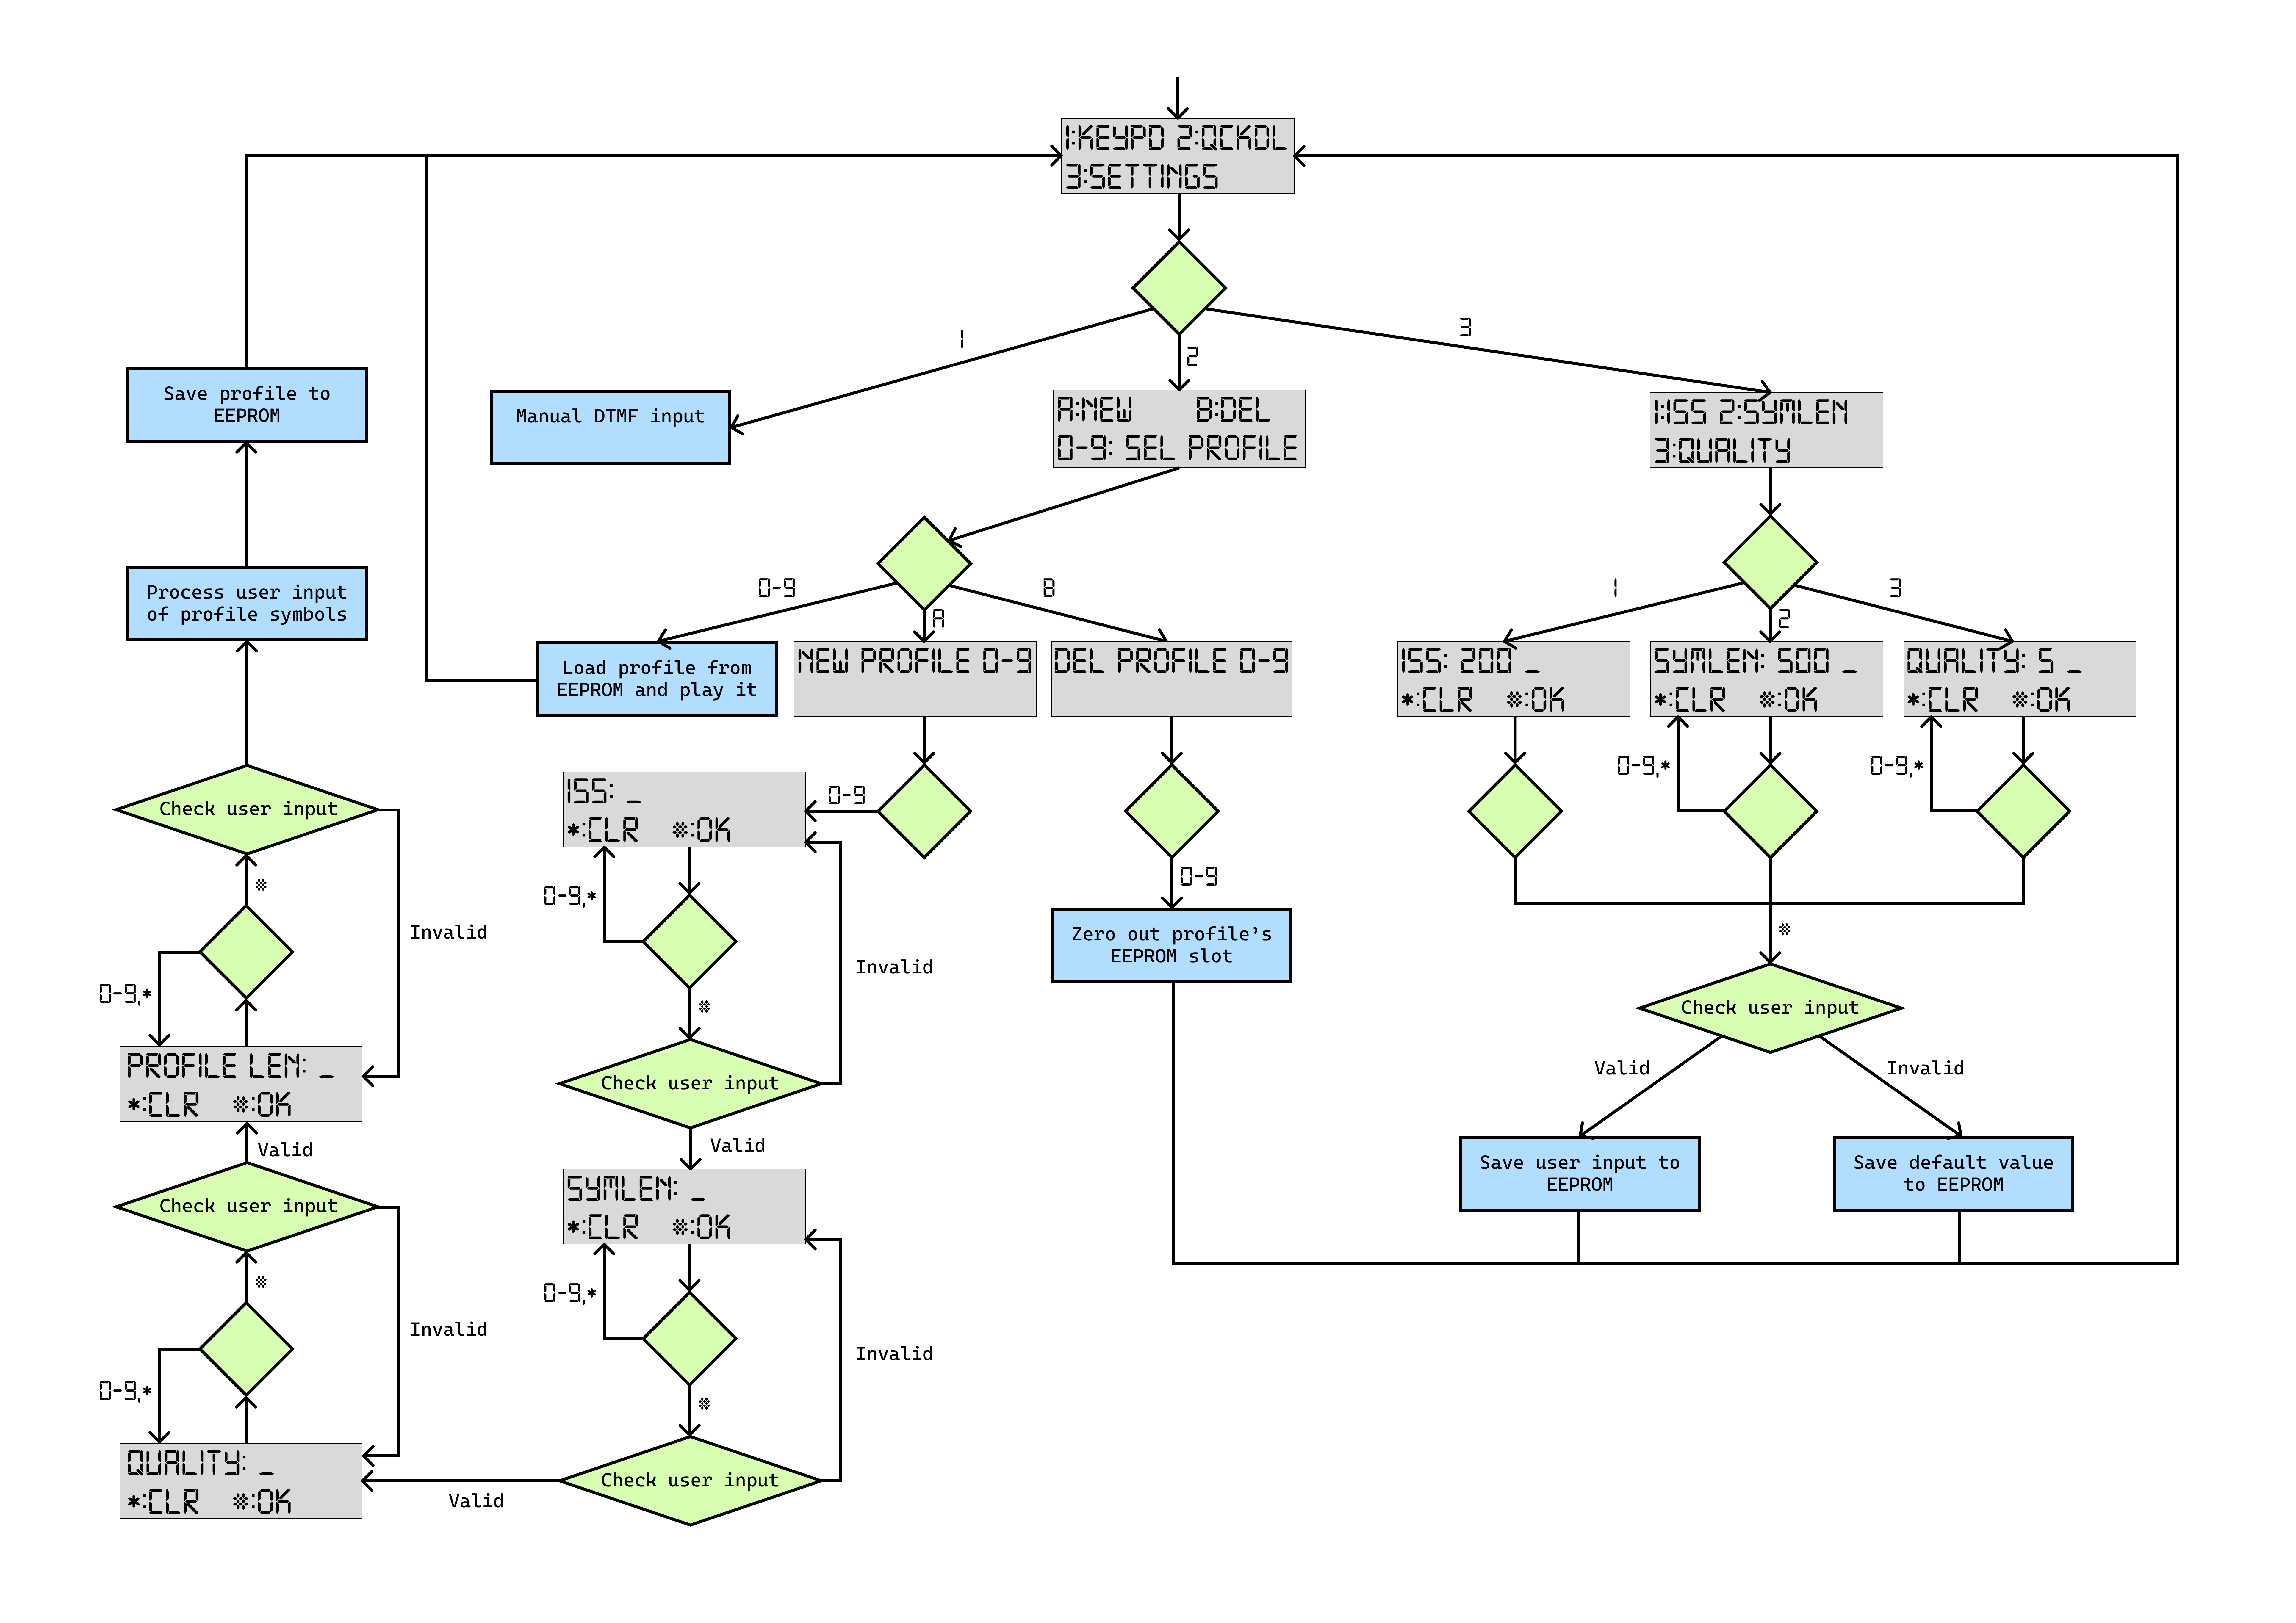
\includegraphics[height=0.67\textheight, angle=90]{system_flow_chart}
      \caption{Flow chart showing system interface. Grey boxes represent the contents of the LCD screen as displayed to the user. Some system actions, such as clearing/displaying user input are omitted for brevity. Keypad input which is ignored by the system is also omitted.}~\label{fig:system-interface}
   \end{figure*}

   Excluding some initial setup, the system is entirely interrupt-based, and the CPU is put in sleep mode (using the \verb!WFI! instruction) while inactive. This approach was found to result in a significant reduction of power consumption. The interrupt-based system has an average current draw of (TODO) (measured over (TODO) minutes of use), whereas the same system with a busy waiting loop in \verb!main! has an average current draw of (TODO) (measured over the same time period).

   The system also uses a number of external circuits which support its operation. These circuits will be discussed in due course below, however a full circuit schematic can be found in Figure~\ref{fig:circuit-schematic}.

   \begin{figure*}
      \centering
      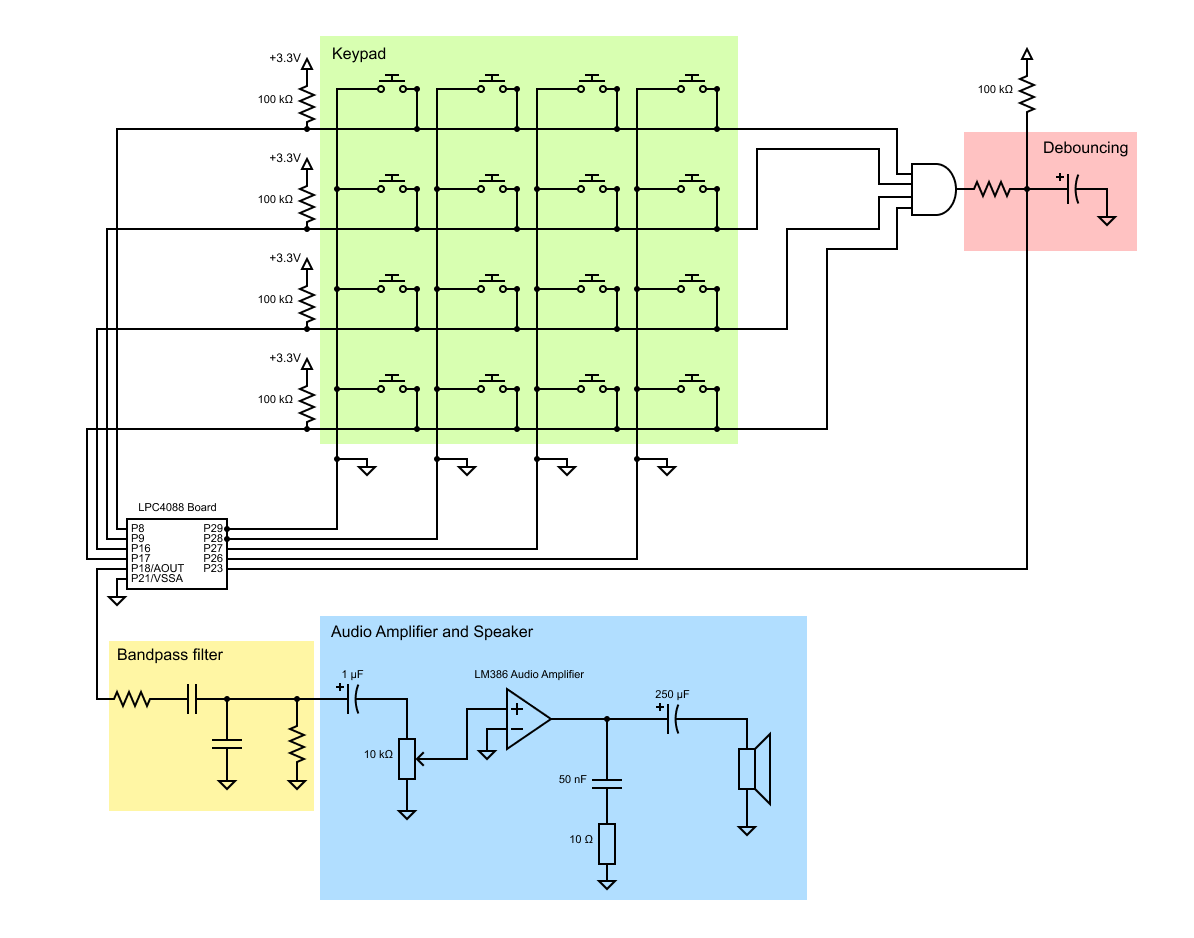
\includegraphics[width=0.8\textwidth]{circuit_schematic}
      \caption{Circuit schematic for the DTMF encoding system.}~\label{fig:circuit-schematic}
   \end{figure*}

   Section \ref{system-design} describes the design of the DTMF encoding system. The system's architecture and separation of concerns is described in subsection \ref{system-arch}. Subsection \ref{dac} describes the implementation of DTMF tone generation. Subsection \ref{keypad} discusses how keypad input is handled. Finally, subsection \ref{settings-quickdial} describes how settings and quickdial are implemented, including the use of EEPROM as a persistent storage medium.

   Section \ref{schedule} outlines a breakdown of the system's implementation into individual tasks, as well as a schedule for implementing these tasks.

\section{System Design}~\label{system-design}

\subsection{System architecture}~\label{system-arch}

To implement a variety of features while adhering to good seperation of concerns, the system makes use of several software components. Code for these components is grouped into one or more source files. These software components, together with their constituent source files are shown in Figure \ref{fig:software_components}.

\begin{figure*}
   \centering
   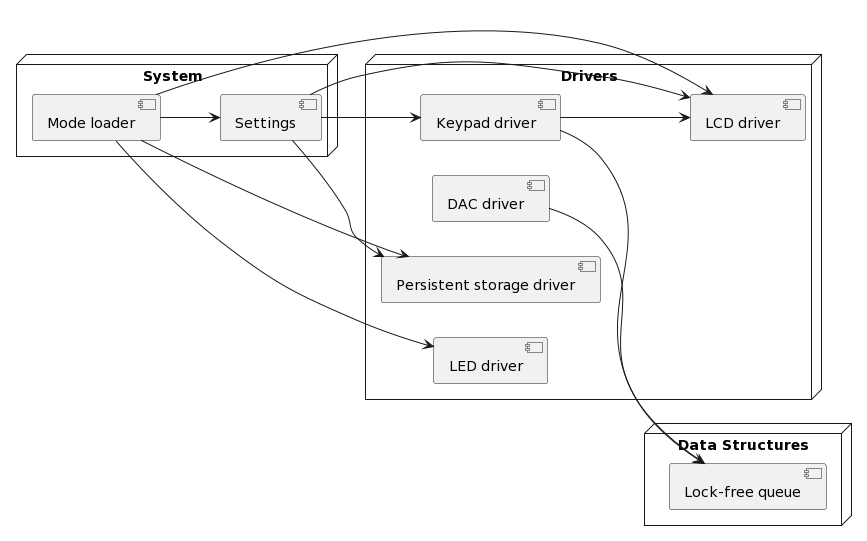
\includegraphics[width=0.92\textwidth]{software_components}
   \caption{Software components for the system. The source files constituting each component are also shown.}
   \label{fig:software_components}
\end{figure*}

The drivers component includes all code that interacts with the board's hardware in a low level way (manipulation of hardware registers). A large portion of this code is sourced from other projects, and adapted for use in our system. Notably, the EEPROM driver was sourced from \href{https://github.com/RT-Thread/realboard-lpc4088/tree/master/software/lpcware_lpc408x/Drivers}{this project}.

The utilities component contains functions for busy waiting a fixed number of milliseconds, or microseconds. These are used in the LCD driver, as well as for software de-bouncing while processing keypad input (see below).

The LCD component provides a high level interface for interacting with the LCD.

The tone generation component contains code that is used to generate samples for the DTMF tones. It also contains a global thread-safe queue which is used to enqueue symbols entered in the keypad, as well as functions which can start the generation of a tone, or enqueue its symbol for later processing. The component is used by quickdial code, as well as in the manual mode of the system.

The keypad component contains code for processing keypad input. This includes an interrupt service routine that is executed when a key press is detected, a function for initializing the GPIO pins used by the keypad, as well as another for customizing the callback called when a key press is registered. The component is used by all system modes to process user input.

The menu component contains utility functions that are used to build menus in settings and quickdial mode, as well as for processing numerical user input.

The settings and quickdial components contain code for each of the two respective modes.

\subsection{DTMF tone generation}~\label{dac}

This section describes the design of code in the tone generation component mentioned above.

Tones are produced using a function called \verb!tone_play_or_enqueue!. 

This function takes a DTMF symbol (in the form of a column and a row), and attempts to start generating its tone by calling another function \verb!dac_interrupt_enable!.

\verb!dac_interrupt_enable! returns a boolean to indicate success or failure. It will fail if another DTMF tone is currently being produced by the system, and succeeds otherwise.

Given that the maximum symbol length and intersymbol spacing are $5$s each, a user can easily enter symbols faster than their tones are produced, and hence the failure of \verb!dac_interrupt_enable! is a common situation that the system has to deal with.

On failure, our system enqueues the symbol passed to \verb!tone_play_or_enqueue! to a global queue, and this is later dequeued by the timer ISR generating the tone when it is done.

\subsubsection{The queue data structure and thread-safety considerations}

The salient point in this discussion is that the system uses a global queue which can be concurrently accessed by consumers and producers (due to interleaving of multiple ISRs and normal code).

To meet the system's needs, the queue needed to support the following operations:
\begin{enumerate}
   \item Enqueue a DTMF symbol.
   \item Check if queue is empty and dequeue. This must be one atomic operation.
\end{enumerate}

Due to concurrent access, the queue also had to be implemented with thread safety in mind, i.e. its operations had to be atomic. However, some simplifying assumptions were made in implementing this queue.

Firsly, concurrent execution of two producers is not possible. In manual mode, tones are enqueued by a GPIO ISR, and since one GPIO ISR cannot preempt another, enqueuing occurs serially in this case. Similarly, in quickdial mode, tones are enqueued in normal mode, and hence the producer code is serial.

Concurrent execution of two consumers is also not possible. Symbols are dequeued by timer ISRs running on a single timer peripheral. It is easy to see that timer interrupts that invoke these ISRs can only happen serially.

Secondly, a fixed size queue was deemed acceptable. This assumption allows us to implement the queue as a circularly indexed array, rather than a more complex linked list data structure. A size of 2048 elements was chosen.

To see why this approach is acceptable, consider the worst case scenario, where both intersymbol spacing and symbol length are each set to their maximum values of $5$s, so that processing of a single symbol takes $10$s. 

It is safe to assume that the most eager user would enter key presses at a rate of not more than $3$ symbols per second. This means that symbols are enqueued at an overall rate of $3 - 1/10 = 2.9$ symbols per second. For the queue to overflow, the user has to continuously enter input for $2048/2.9 = 706$ seconds, or more than $11$ minutes.

This was deemed to be an unlikely situation. Note however, that were the queue to overflow, there would not be a catastrophic failure of the system; instead the oldest entered symbols would simply be discarded.

Although this implementation approach significantly simplifies code, and may also be more performant than a linked list approach (which would resort to a \verb!malloc! implementation for allocating nodes), one downside is that the statically allocated queue takes up a significant portion of memory, while being mostly under-utilized.

The thread safe queue operations were implemented using hardware synchronization. The ARMv7-M architecture provides \verb!LDREX! (load exclusive) and \verb!STREX! (store exclusive) instructions for this purpose.

When a load exclusive instruction is used, a hardware monitor tracks subsequent stores to a small block containing the loaded address using a tag. Once a single exclusive store to the block has been executed, the monitor prevents subsequent exclusive stores before another exclusive load is performed.\cite{armv7_m_architecture_manual}

The use of these instructions required the queue to be implemented in ARM assembly (inline assembly is discouraged when using exclusive load/store instructions\cite{compiler_migration_guide}).

Pseudo-code for the two operations implemented is shown in Listing~\ref{alg:enqueue} and Listing~\ref{alg:check_dequeue} respectively. A line marked as \textbf{atomic}, or a section marked \textbf{critical-section} indicate code which is protected by \verb!LDREX!/\verb!STREX! guards. Note also that thread safety can be achieved simply by guarding access to a single, additional shared variable; the queue size. This is possible because there is only one producer and one consumer that concurrently access the queue, so it is impossible for the queue's head or tail index variables to be shared.

\begin{algorithm}
   \caption{Pseudocode for the lock-free queue's enqueue operation. Note the atomic increment of $N$}\label{alg:enqueue}
   \KwData{
      \begin{itemize}
         \item $q$ is the queue array
         \item $tail$ is the immediate index after the last element in the queue
         \item $s$ is the symbol to be enqueued
         \item $N$ is the number of items in the queue
         \item $M$ is the queue size (maximum capacity of the queue)
      \end{itemize}}
      \textbf{atomic} $N \gets (N + 1) \bmod M$; \\
      $q[tail] \gets s$; \\
      $tail \gets (tail + 1) \bmod M$;
\end{algorithm}

\begin{algorithm}
   \caption{Pseudocode for the lock-free queue's check and dequeue operation.}\label{alg:check_dequeue}
   \KwData{
      \begin{itemize}
         \item $q$ is the queue array
         \item $head$ is the index of the start of the queue
         \item $N$ is the number of items in the queue
         \item $M$ is the queue size (maximum capacity of the queue)
         \item $default$ is the smallest integer value ($-2^{31}$).
      \end{itemize}}
      \CritSection{
         $tmp \gets N$;\\
         \If{$tmp = 0$}
         {
             $N \gets (tmp - 1) \bmod M$\;
         }
      }
      $res \gets default$;\\
      \If{$tmp \ne 0$}
      {
         $res \gets q[head]$;\\
         $head \gets (head + 1) \bmod M$;
      }
\end{algorithm}

There is one more place where the system requires considerations of thread safety. In \verb!dac_interrupt_enable!, the code requires a way of knowing whether a tone is playing or not, in order to succeed or fail in starting the next tone. For this purpose, a global variable \verb!dac_interrupt_flag! is used. This flag is set when a timer interrupt is enabled, and reset when one is disabled.

However, when \verb!dac_interrupt_enable! checks the global flag, the following data race can occur:
\begin{enumerate}
   \item First, \verb!dac_interrupt_flag!, which happens to have a value of $1$, is loaded from memory into a register.
   \item Next, the thread of execution running \verb!dac_interrupt_enable! is preempted by a timer interrupt.
   \item The timer ISR invoked happens to be the one at the end of tone generation. It checks the queue, which happens to be empty, resets \verb!dac_interrupt_flag! and exits.
   \item \verb!dac_interrupt_enable! continues executing with the wrong value for \verb!dac_interrupt_flag!, resulting in an unneeded failure.
\end{enumerate}

This sequence of events will prevent a tone from being generated for the entered symbol. Instead, it is enqueued, and its tone may be produced after the next entered symbol is processed.

In order to prevent this data race, \verb!dac_interrupt_flag! is accessed using an atomic test-and-set in \verb!dac_interrupt_enable!. The compiler builtin \verb!__sync_lock_test_and_set! is used to implement this atomic test-and-set.

\subsubsection{Algorithm used for generating DTMF tone samples}

DTMF tones consist of a composition of two sine waves whose frequency is determined by the row and column index of the corresponding DTMF symbol.

The sine function is fairly computationally intensive, and hence our system precomputes samples for one period of a sine wave, storing them in a lookup table. The table is filled in each time the system enters manual mode, or loads a quickdial profile. The number of samples in the table is determined by the quality setting, which is log base $2$ of the size. This means that the size ranges from $16$ to $512$ samples. The exact relationship between the size of the lookup table and the quality of the tone produced will be discussed below.

In what follows, $LUT$ represents the lookup table, $N$ its size, and $f_1$ and $f_2$ are the higher and lower frequencies of a DTMF tone.

In order to make the most efficient use of the sine lookup table, the frequency of the timer interrupt is set to $4$ times the highest frequency of the DTMF tone being produced. This means that one of the sine waves can be produced simply by repeatedly getting the $0\textsuperscript{th}$, $N/4\textsubscript{th}$, $N/2\textsuperscript{th}$ and $3N/4\textsubscript{th}$ samples from the lookup table in each invocation of the ISR. 

Note that since the DTMF tone signal has a frequency spectrum bandlimited by $f_1$, the Nyquist criterion specifies that the lower bound on the sampling frequency of the signal should be $2f_1$. In this case, we are using a sampling frequency of $4f_1$, which is fairly close. The relationship between sampling frequency and $f_1$ was determined empirically.

Samples for the lower frequency sine component of the DTMF tone are determined using the following equation:
\begin{equation}
   \label{eqn:low-f-dtmf-sine}
   \frac{1}{2}\Bigg(LUT\bigg[\bigg\lfloor\frac{f_2i}{f_1}\bigg\rfloor \bmod N\bigg] + LUT\bigg[\bigg\lceil\frac{f_2i}{f_1}\bigg\rceil \bmod N\bigg]\Bigg)
\end{equation}
where $i$ is a global variable (called \verb!sample_index! in the code) which keeps track of the tone generation progress in between timer ISR invocations, and is incremented by $N/4$ each time the timer ISR is invoked.

Equation~\ref{eqn:low-f-dtmf-sine} essentially finds the two samples that lie on either side of the sine value required, and then averages them. This is why increasing the size of the lookup table improves the quality of the tone produced; it improves the precision of the result computed by this average.

We can quantify the error in approximating sine by Equation~\ref{eqn:low-f-dtmf-sine} to show that the quality setting has a tangible effect on the resolution of the tone produced. It is easy to see that the error is given by
$$ E(x) = \bigg|\frac{1}{2}\bigg[\sin(x + \epsilon_1) + \sin(x - \epsilon_2)\bigg] - \sin(x)\bigg| $$
where $\epsilon_1, \epsilon_2 \ge 0$ and $\epsilon_1 + \epsilon_2 = \frac{2\pi}{N}$

Using trigonometric identities, this error can be expressed as
\begin{equation*}
E(x) = \frac{1}{2}\bigg|[\cos(\epsilon_1) + \cos(\epsilon_2) - 2]\sin(x) + [\sin(\epsilon_1) + \sin(\epsilon_2)]\cos(x)\bigg|
\end{equation*}

Since $\epsilon_1, \epsilon_2$ are fairly small, we can assume to first approximation that $\epsilon^n \approx 0$ for $n \ge 2$, and furthermore we can use Taylor series to approximate the error as
$$ E(x) \approx \frac{1}{2}\bigg|[\epsilon_1 + \epsilon_2]\cos(x)\bigg| \le \frac{\pi}{N} $$

For the minimum quality setting, $N = 16$, and hence the \textbf{total} relative error in the DTMF tone sample is bounded by $\frac{\pi}{2\times 16} \approx 0.098$ (we divide by $2$ because the lower frequency component contributes to half the amplitude of the DTMF tone). This corresponds to a maximum error equal to about $10\%$ the amplitude of the signal. Since the DAC has a resolution of $10$ bits, and $0.098 \times 1024 \approx 100 \gg 1$, this error easily manifests itself as audible noise. 

For the maximum quality setting, $N = 512$, so the total relative error is bounded by $\frac{\pi}{2\times 512} \approx 0.0031$. This corresponds to a maximum error equal to about $0.3\%$ of the signal. The error noise is still theoretically audible in the DAC output, as $0.0031 \times 1024 \approx 3.14 > 1$, however it is far less than the minimum quality setting.

One note about the implementation of Equation~\ref{eqn:low-f-dtmf-sine}; integer division in a computer is the floor of the real result when the latter is positive, as in the above case. Ceiling division is accomplished using the following formula\cite{warren2012hacker}:
$$ \bigg\lceil \frac{x}{y} \bigg\rceil = -\bigg\lfloor -\frac{x}{y} \bigg\rfloor $$

A number of optimizations were applied to the formula for the lower frequency sine component. Firstly, $N$ is fixed to be a power of $2$ (recall that the quality setting is $\log_2 N$), and hence the modulo operation can be replaced by a bitwise and, using the following formula that works when $y$ is a power of two:
$$ x \bmod y = x \,\,\&\,\, (y - 1) $$

Secondly, the two divisions by $f_1$ are costly, but avoidable. By having one version of the timer ISR for each possible tone, the divisions become constant, allowing them to be optimized into a shift and a multiplication by the compiler\cite{warren2012hacker}. In order to implement this specialization cleanly, \verb!timer_callback_isr! is declared as \verb!STATIC_INLINE! (encouraging the compiler to inline its body), and macros are used to define specialized wrappers for it, for example \verb!timer_callback_isr_1209_697!. Function pointers to these specialized wrappers are stored in a 2-dimensional \verb!dispatch_table! variable, with the pointer at a particular 2-dimensional index pointing to the wrapper that produces the tone with the corresponding row and column index. This arrangement has additional benefits, namely the elimination of global state that would have to keep track of what tone is being produced in between invocations of the timer ISR.

\subsubsection{Chaining of DAC interrupts}

Earlier, it was mentioned that the timer ISR checks if tone generation has finished, and attempts to start generating a new tone if this is the case. This is done at the end of \verb!timer_callback_isr!, by comparing the value of \verb!sample_index! with $f_1 \times N \times \text{symbol length in seconds}$.

If the latter check succeeds, the tone has been generated for the duration determined by the system's symbol length setting, and \verb!timer_callback_isr! calls \verb!timer_set_callback_delay!. This function takes a callback and a delay (in CPU cyles), and sets up the timer to call this callback after the given delay. Since the same timer peripheral is used for driving the DAC and for the delayed callback, this call simultaneuosly disables \verb!timer_callback_isr! from being invoked again. The delay used is determined by the system setting for intersymbol spacing. The callback used in this case is \verb!pop_and_dac_interrupt_enable!.

This function dequeues any existing symbol in the queue, and enables generation of its tone. Since it is only used by \verb!timer_callback_isr!, there is no need to check \verb!dac_interrupt_flag!, as it must be set when the function is called. Hence the function enables generation of the tone by calling \verb!dac_interrupt_enable_unsafe!, a version of \verb!dac_interrupt_enable! that skips checking or setting \verb!dac_interrupt_flag!. (Since \verb!dac_interrupt_enable_unsafe! is a subset of \verb!dac_interrupt_enable!'s functionality, the latter function wraps the former.) 

There is a sequence of events where this implementation suffers from a data race:
\begin{enumerate}
   \item \verb!tone_play_or_enqueue! is called due to a key press, or playback of a quickdial profile, while another tone has just finished being produced, and a delay is in place after which \verb!pop_and_dac_interrupt_enable! will be called.
   \item The check of \verb!dac_interrupt_flag! (inside \verb!dac_interrupt_enable!) indicates that a tone is currently being generated, so \verb!dac_interrupt_enable! returns unsuccessfully.
   \item At this point, the timer interrupt preempts execution. The queue happens to be empty (the symbol has not yet been enqueued), and so \verb!pop_and_dac_interrupt_enable! determines that no other tone needs to be generated.
   \item Execution of the other thread resumes. Since \verb!dac_interrupt_enable! failed, the symbol is enqueued, and its tone is not produced. 
\end{enumerate}

This data race is very hard to avoid, as it manifests itself due to the preemption of code execution by a timer interrupt. 

For manual mode, one solution could be to set the priority level of GPIO interrupts and timer interrupts to be the same. This would prevent the timer interrupt from preempting execution of \verb!dac_interrupt_enable! inside the keypad ISR. However, it would not solve the issue in the case of quickdial mode.

Another solution would be to disable timer interrupts in the critical section between checking \verb!dac_interrupt_flag!, and enqueuing the tone.

Given that the critical section is short (less than 10 instructions), and is executed infrequently, the sequence of events described above is very unlikely. Due to the inelegance of possible solutions considered, it was chosen to avoid handling this improbable error situation robustly.

\subsubsection{Smoothing using the bandpass filter}

The DAC output changes discontinuously when it is updated. This imparts jagged edges to the produced signal, which translates to audible high frequency artifacts. Given the narrow frequency range of DTMF tones, a simple analog low pass filter can be used to effectively remove these artifacts, resulting in cleaner sound output. 

In addition, the bouncing from keypad presses can cause small, but audible low frequency noise artifacts in the audio output of the system. This can also be mitigated by using a simple high pass filter.

Both sources of noise were significantly reduced in the final system through the use of a bandpass filter, which only lets through frequencies in a narrow range around the DTMF tone frequencies. This circuit processes the output from the DAC and its output is fed into a simple analog audio amplifier, and its details are shown in Figure~\ref{fig:circuit-schematic}.

\subsection{Keypad input} \label{keypad}

\subsubsection{Keypad circuit and polling loop}

The keypad's button switches are organized in a grid as shown in the schematic of Figure~\ref{fig:circuit-schematic}. Each of the keypad's rows and columns are connected to GPIO pins on the microcontroller board.

A polling loop is required to register key presses. Pseudocode for such a loop is shown in Listing~\ref{alg:polling-loop}. Column pins act as outputs initially set high, while the row pins are inputs set to $V_{CC}$ using a pull up resistor. Each column pin is then set low in turn. If any of the keypad switches are closed, current can flow from the switch's row pin to its column pin, resulting in a voltage drop across the row pin's pull up resistor, and setting the state of that pin to low. The key press can then be detected by simply checking each row pin to see if it is low. The delays after setting column pins ensure that the state of each pin is allowed to settle before reading the row pins.

\begin{algorithm}
   \caption{Pseudocode for the polling loop used to detect key presses}\label{alg:polling-loop}
   \KwData{
      \begin{itemize}
         \item $P_{col, i}$ is the GPIO pin for the $i\textsuperscript{th}$ column.
         \item $P_{row, i}$ is the GPIO pin for the $i\textsubscript{th}$ row.
      \end{itemize}}
      \For{$i \in \{1, 2, 3, 4\}$}{
         \textbf{set} $P_{col, i}$ to $0$;\\
         \textbf{delay} $100$ $\mu$s;\\
         \For{$j \in \{1, 2, 3, 4\}$}{
            \If{$P_{row, j} = 0$}{
               Keypress detected at column $i$, row $j$.
            }
         }
         \textbf{set} $P_{col, i}$ to $1$;\\
         \textbf{delay} $100$ $\mu$s;
      }
\end{algorithm}

In our code, the polling loop is encapsulated in a function \verb!read_keypad!, which is triggered on a pin interrupt as described below. The function also contains some logic for disabling pin interrupts on the keypad while the polling loop is being executed, and re-enabling them afterwards. In addition, on detecting a key press, this function calls the callback indicated by a global function pointer \verb!read_keypad_callback!, which takes as parameters the row and column of the key. This allows the keypad code to be customized for use in various settings, by simply changing the value of this pointer (using an additional function \verb!keypad_set_read_callback!).

\subsubsection{Keypad interrupts}

Keypad input is detected using GPIO interrupts. By setting all of the column pins low, and configuring all of the rows as inputs pulled up to $V_{CC}$, a key press will manifest as a falling edge at the row pin of the key (as current can flow from the row to the column pin, and there is a voltage drop across the pull up resistor). By setting a GPIO interrupt to trigger on such a falling edge, key presses can be detected and handled using interrupts.

Due to limitations of the board used, at most two GPIO pins can be used to trigger interrupts on a falling edge. For this reason, an AND gate was used to combine the state of all of the row pins, feeding the output to a single, interrupt pin that triggers on a falling edge. This setup is shown in Figure~\ref{fig:circuit-schematic}. It is easy to see using boolean logic that such a setup will cause a falling edge at the interrupt pin whenever there is a falling edge at one or more row pins. Hence an interrupt will trigger whenever one or more keys on the keypad is pressed.

Note that while this interrupt scheme can detect the press of one or more keys, it cannot determine which key was actually pressed. This responsibility is delegated to the polling loop in the ISR (which is the \verb!read_keypad! function described above). A basic assumption of this scheme is that a human user will press the key for a longer duration of time than it takes for the interrupt to be detected and handled.

\subsubsection{Debouncing}

Digital inputs can suffer from a phenomenom called bouncing, where sudden changes in the physical state of the attached circuit (e.g. current flow after closing a switch) cause voltage fluctuations, which in turn causes the state of the digital input to bounce between high and low before settling on a stable value. 

In the case of the polling loop, setting the state of column pins in software can cause bouncing, however this is dealt with by introducing a small delay after each change in an output pin, as discussed above.

Bouncing at the interrupt pin after a keypad switch is pressed is more problematic, however, as it can cause several transient falling edges, resulting in multiple interrupts being registered. Since there is no obvious way to deal with this in software, a hardware debouncing circuit was implemented and attached to the interrupt pin. This circuit is shown in Figure~\ref{fig:circuit-schematic}, and is effectively a simple RC lowpass filter. The RC values determine the frequency of bouncing which the filter can remove, and were determined empirically for the keypad used.

An RC lowpass filter works as a debouncing circuit because bouncing can be interpreted as high frequency noise added to a reverse unit step function (the falling edge). Unfortunately, the falling edge contains high frequency components which are also filtered out by the circuit, and so the filter effectively smooths the transition from high to low. If the RC values are chosen carelessly, the output of the switch is smoothed to the extent that an interrupt will not trigger when the key is pressed, or the delay between pressing a key and the polling loop that detects that key makes the system appear unresponsive, or results in lost key presses (as mentioned above).

\subsection{Settings and Quickdial} \label{settings-quickdial}

\subsubsection{Settings mode}

As mentioned above, the user can set system settings via a settings mode, which, as shown in Figure~\ref{fig:system-interface} can be accessed by pressing $2$ after booting the system. In this mode, the user can set the intersymbol spacing, symbol length, and quality used by the system.

While entering the value for a system setting, the user can clear their input by pressing the * key.

After entering a value for a particular setting, the user presses the \# key to submit their option. This redirects them to the boot menu. Valid user inputs are applied to the global variable \verb!settings! used by the system, and stored to EEPROM in a fixed location, for use when the system is rebooted. Invalid user inputs (ones which do not fall in the allowed range for that setting as specified in Section~\ref{introduction}) are silently rejected (not applied or stored).

In the code, settings are represented by a \verb!Settings! struct containing all configurable fields, as well as a checksum for dealing with EEPROM corruption (see below).

\subsubsection{Quickdial mode}

In quickdial mode, the user can create, load and delete profiles. These are sequences of at most $32$ DTMF symbols, with their own, embedded settings for playback. Profiles are represented by a \verb!Profile! struct, which includes a \verb!Settings! field, a profile length, a \verb!char! array holding the profile's symbols, and a checksum for dealing with EEPROM corruption (see below).

Profiles are assigned by the user to keys $0-9$, allowing for a maximum of $10$ saved profiles. When the user enters quickdial mode, they can load a profile by pressing keys $0-9$, create (or overwrite) a profile by pressing A, and delete a profile by pressing B, as shown in Figure~\ref{fig:system-interface}.

Attempting to load a non-existent or corrupted profile prompts a ``\verb!Loading failed!'' message to the user, and returns them to the boot menu. 

Loading an existing, valid profile applies the profile's settings to the system (by assigning to the global \verb!settings! variable), plays back the profile, and then returns the user to the boot menu. Playback uses the same \verb!tone_play_or_enqueue! function as manual mode. Since this is interrupt based, busy waiting (\verb!delay_ms!) is used in normal mode to ensure that the playback has finished before returning the user to boot mode. The required delay is calculated from the profile length, and symbol length/intersymbol spacing settings of the profile. A $500$ ms overhead is added to ensure that playback finishes before the delay expires.

When the user creates a new profile, they are prompted to enter each of the fields in the \verb!Profile! struct in turn (excluding the checksum). If the user enters an invalid input for any of the settings or the profile length, their input is cleared, and they are prompted to enter a new value for the field. The user can also clear their input manually by pressing the * key.

The value entered for profile length is used in the menu where the user enters symbols for the profile to determine when to stop registering new symbols. After successfully entering all the details of a profile, the latter is stored to EEPROM, and the user is redirected to the boot menu.

Users can also delete their profiles. This works by zeroing out the region of EEPROM allocated to that profile.

\subsubsection{Using the EEPROM}

Our system makes use of EEPROM by writing the bytes of \verb!Settings! or \verb!Profile! structs directly to it. This simple serialization strategy requires that these structs contain only flat fields (no pointers). System settings, and the 10 quickdial profiles are each written to their own, hardcoded region in the EEPROM.

Data read from and written to EEPROM can be corrupted. In order to detect corruption, the structs stored to EEPROM have a checksum field. This is set to a bitwise exclusive or of all other fields before storing the struct to EEPROM. Note that in the case of \verb!Profile! structs, the checksum of the embedded \verb!Settings! struct is not included in the checksum for the \verb!Profile!, as this would cancel out the contribution to the checksum from the rest of the \verb!Settings! fields.

When loading from EEPROM, the checksum is re-computed and checked against the stored version. Structs with corrupted checksums are discarded. In the case of settings, the defaults are used instead. In the case of loading a profile, the load simply fails.

This lax approach to error handling is tolerated because the system is not expected to store valuable information. Lost data, i.e. system settings or quickdial profiles, can be restored with minor inconvenience to the user.

In order to deal with the unlikely possibility that a struct is corrupted without invalidating the checksum, or to deal with cases where the checksum is valid while the data is not\footnote{This occurs, for example, when booting the system after the EEPROM has been erased. The region containing system settings is zeroed out, so the checksum check will succeed ($0 \oplus 0 = 0$), but the data is invalid.}, the system also checks that values for any settings (even those embedded in a quickdial profile) are in a valid range before loading them. When loading system settings, invalid fields are set to the default value. In the case of profiles, invalid fields in the embedded settings cause profile loading to fail.

\section{Management} \label{schedule}
\subsection{Final Deadline}
The final deadline will be set to \textbf{10\textsuperscript{th} May} to ensure that the work is done at a proper pace whilst leaving enough room for any necessary 
adjustments.

\subsection{Tasks}
To implement the system, the above-mentioned software components have to be split into multiple sub-tasks. Each task will have a fairly allocated time-frame for completion. The deadlines for each task are as follows:
\subsubsection{Drivers}
\begin{enumerate}
    \item LCD Driver - Deadline: \textbf{8\textsuperscript{th} April}. Subtasks: Symbol and C-String to LCD function, Display function.
    \item Keypad Driver - Deadline: \textbf{8\textsuperscript{th} April}. Subtasks: Polling Cycle function for the keypad, Keypad driven interrupt.
    \item LED Driver - Deadline: \textbf{8\textsuperscript{th} April}. Subtasks: LED On function, LED Off function.
    \item Persistent Storage Driver - Deadline: \textbf{16\textsuperscript{th} April}. Subtasks: Serialising Data, Persisting Data, Loading Data, Deserializing Data.
    \item DAC Driver - Deadline: \textbf{20\textsuperscript{th} April}. Subtasks: Timer interrupt handler enable method, Set timer duration function, Interrupt handlers.
\end{enumerate}

\subsubsection{Data Structures}
\begin{enumerate}
    \item Lock-Free queue - Deadline: \textbf{1\textsuperscript{st} April}. Subtasks: Atomic Enqueue function, Atomic Check and Dequeue function.
\end{enumerate}

\subsubsection{System}
\begin{enumerate}
    \item Mode loader - Deadline: \textbf{16\textsuperscript{th} April}. Subtasks: Display Options function, Load settings/normal mode functions.
    \item Settings Mode - Deadline: \textbf{27\textsuperscript{th} April}. Subtasks: Display settings function, Save settings function.
\end{enumerate}

\subsection{Task Dependencies}
When considering the inter-dependencies of the tasks listed above, there is a discrete order of task development that when followed should ensure that each subsequent task has adequate resources to be accomplished. The order is the following:
\begin{enumerate}
    \item Lock-Free Queue
    \item LCD Driver
   \item LED Driver
   \item Keypad Driver
   \item Persistent Storage Driver
   \item DAC Driver
\end{enumerate}

\section{Closure}

In conclusion, this document describes the design of an efficient and robust system implementing DTMF encoding, as well as a number of auxiliary features. The system's software has been split up
into modules, showing good separation of concerns. Special considerations were made to ensure thread safety of the system, and an efficient algorithm was used to generate DTMF tone samples. The circuit provided in the handbook was augmented to improve the quality of the system's output. 

\bibliographystyle{ieeetr}
\bibliography{references}

\end{document}
